\documentclass[aspectratio=169]{beamer}
\usetheme{Madrid}
\usecolortheme{default}

\usepackage[utf8]{inputenc}
\usepackage[T1]{fontenc}
\usepackage{tikz}
\usepackage{hyperref}
\usepackage{fontawesome5}

\usetikzlibrary{shapes.geometric, arrows, positioning}

\definecolor{kivablue}{RGB}{41,128,185}
\definecolor{kivagreen}{RGB}{39,174,96}
\definecolor{kivaorange}{RGB}{230,126,34}
\definecolor{kivared}{RGB}{231,76,60}
\definecolor{kivagray}{RGB}{127,140,141}

\setbeamercolor{structure}{fg=kivablue}
\setbeamercolor{palette primary}{bg=kivablue,fg=white}
\setbeamercolor{palette secondary}{bg=kivagreen,fg=white}
\setbeamercolor{palette tertiary}{bg=kivaorange,fg=white}

\title[KIVA Setup \& Play]{Get KIVA Running \& Start Playing}
\subtitle{No technical experience needed}
\author{MA AI Hub x SundAI Pre-Session}
\date{May 6, 2026}

\begin{document}

\begin{frame}
\titlepage
\end{frame}

% ============================================================
% PART 1: INSTALLATION
% ============================================================

\begin{frame}{Before You Start -- Check These}
\begin{columns}[T]
\column{0.5\textwidth}
\textbf{\faApple\ Mac users}
\begin{itemize}
    \item Any Mac with Apple Silicon (M1/M2/M3) works great
    \item Open \textbf{Terminal} app (Cmd+Space, type ``Terminal'')
\end{itemize}

\column{0.5\textwidth}
\textbf{\faLinux\ Linux users}
\begin{itemize}
    \item Ubuntu 20.04+ recommended
    \item Open your terminal app
\end{itemize}
\end{columns}

\vspace{0.5cm}

\begin{alertblock}{\faExclamationTriangle\ Windows is not supported}
If you only have Windows, use the \textbf{GitHub Codespace} option (we'll help you set it up).
\end{alertblock}

\vspace{0.3cm}

\textbf{You will need:}
\begin{itemize}
    \item An \textbf{OpenAI API key} -- get one at \url{https://platform.openai.com/api-keys}
    \item \textbf{Google Chrome} browser (version 134 or newer)
\end{itemize}
\end{frame}

\begin{frame}{Step 1 of 6: Download KIVA}
Open your terminal and paste this line, then press Enter:

\vspace{0.3cm}

\begin{center}
\large \texttt{git clone https://github.com/sensein/riverst.git}
\end{center}

\vspace{0.3cm}

Then type:

\vspace{0.1cm}

\begin{center}
\large \texttt{cd riverst}
\end{center}

\vspace{0.5cm}

\begin{block}{What just happened?}
You downloaded the entire KIVA project to your computer and moved into its folder.
\end{block}
\end{frame}

\begin{frame}{Step 2 of 6: Create a Python Environment}
Paste these \textbf{3 lines one at a time}, pressing Enter after each:

\vspace{0.3cm}

\begin{enumerate}
    \setlength\itemsep{0.4cm}
    \item \texttt{cd src/server}
    \item \texttt{conda create -n riverst python=3.11 -y}\\
          {\small\textcolor{kivagray}{(This downloads Python. It takes 1--2 minutes. Wait for it to finish.)}}
    \item \texttt{conda activate riverst}\\
          {\small\textcolor{kivagray}{(You should see ``(riverst)'' appear at the left of your terminal prompt.)}}
\end{enumerate}

\vspace{0.3cm}

\begin{alertblock}{Don't have conda?}
Install it first: \url{https://docs.conda.io/en/latest/miniconda.html}\\
Download Miniconda, install it, then come back here.
\end{alertblock}
\end{frame}

\begin{frame}{Step 3 of 6: Install Server Packages}
Paste these \textbf{2 lines one at a time}, pressing Enter after each:

\vspace{0.3cm}

\begin{enumerate}
    \setlength\itemsep{0.5cm}
    \item \texttt{conda install -c conda-forge ffmpeg -y}\\
          {\small\textcolor{kivagray}{(Audio processing tool. Takes 1--2 minutes.)}}
    \item \texttt{pip install -r requirements.txt}\\
          {\small\textcolor{kivagray}{(All Python dependencies. Takes 2--5 minutes.)}}
\end{enumerate}

\vspace{0.3cm}

\begin{block}{Wait for each command to finish}
You'll see a lot of text scrolling by. That's normal. Wait until the prompt returns before pasting the next line.
\end{block}
\end{frame}

\begin{frame}{Step 4 of 6: Add Your API Key}
Paste this line and press Enter:

\vspace{0.1cm}

\begin{center}
\large \texttt{cp env.example .env}
\end{center}

\vspace{0.2cm}

Now open the file \texttt{.env} in any text editor (VS Code, nano, TextEdit):

\begin{center}
\large \texttt{nano .env}
\end{center}

\vspace{0.2cm}

Find the line that says \texttt{OPENAI\_API\_KEY=""} and paste your key between the quotes:

\vspace{0.1cm}

\begin{center}
\texttt{OPENAI\_API\_KEY="sk-proj-abc123..."}
\end{center}

\vspace{0.1cm}

Save and close (in nano: Ctrl+X, then Y, then Enter).
\end{frame}

\begin{frame}{Step 5 of 6: Install the Frontend}
Open a \textbf{new, second terminal window} and paste these lines one at a time:

\vspace{0.3cm}

\begin{enumerate}
    \setlength\itemsep{0.5cm}
    \item \texttt{cd riverst/src/client/react}
    \item \texttt{npm install}\\
          {\small\textcolor{kivagray}{(Downloads web app dependencies. Takes 1--3 minutes.)}}
\end{enumerate}

\vspace{0.3cm}

\begin{block}{Don't have npm?}
Install Node.js first: \url{https://nodejs.org/} (download the LTS version)
\end{block}
\end{frame}

\begin{frame}{Step 6 of 6: Start KIVA!}
You need \textbf{two terminal windows} running at the same time.

\vspace{0.2cm}

\begin{columns}[T]
\column{0.5\textwidth}
\begin{block}{Terminal 1 (Server)}
\small
\texttt{cd riverst/src/server}\\
\texttt{conda activate riverst}\\
\texttt{python main.py}\\[0.2cm]
\textcolor{kivagray}{\footnotesize Wait for ``Uvicorn running on...''}
\end{block}

\column{0.5\textwidth}
\begin{block}{Terminal 2 (Client)}
\small
\texttt{cd riverst/src/client/react}\\
\texttt{npm run dev}\\[0.2cm]
\textcolor{kivagray}{\footnotesize Wait for ``Local: http://localhost:5173''}
\end{block}
\end{columns}

\vspace{0.3cm}

\begin{alertblock}{Start the server FIRST!}
Terminal 1 must show ``Uvicorn running'' before you run Terminal 2.
\end{alertblock}

\vspace{0.2cm}

\begin{center}
\large Open Chrome and go to: \texttt{http://localhost:5173}
\end{center}
\end{frame}

% ============================================================
% PART 2: WHAT YOU CAN DO WITH KIVA
% ============================================================

\begin{frame}{What Can You Do With KIVA?}
Once KIVA is running, the homepage shows you \textbf{4 categories of activities}:

\vspace{0.3cm}

\begin{enumerate}
    \setlength\itemsep{0.4cm}
    \item \textbf{\faUserFriends\ Avatar customization} -- Pick or create your avatar
    \item \textbf{\faGamepad\ Playground} -- Free chat or a quick demo
    \item \textbf{\faBookReader\ KIVA activities} -- Audiobooks \& vocabulary training
    \item \textbf{\faGlobe\ L2 learning} -- English or Italian as a second language
\end{enumerate}

\vspace{0.3cm}

\begin{block}{Start here}
Click \textbf{``Select your avatar''} first, then try \textbf{``Demo ready to go''}.
\end{block}
\end{frame}

\begin{frame}{Quick Start: Avatar + Demo in 5 Clicks}
\begin{enumerate}
    \setlength\itemsep{0.5cm}
    \item Click \textbf{``Select your avatar''}
    \item Click on \textbf{Fabio} or \textbf{Bruce} to choose one
    \item Click \textbf{Back} to return to the homepage
    \item Under ``Playground'', click \textbf{``Free style interaction''}
    \item Click \textbf{``Run a demo''} $\rightarrow$ allow microphone $\rightarrow$ start talking!
\end{enumerate}

\vspace{0.3cm}

\begin{block}{Tip}
Use \textbf{Chrome} and make sure your microphone is enabled. The avatar listens and responds in real time.
\end{block}
\end{frame}

\begin{frame}{Create Your Own Custom Session}
The \textbf{``Free style interaction''} activity lets you customize your avatar's behavior.

\vspace{0.2cm}

When you click it, you see a form with these key fields:

\vspace{0.2cm}

\begin{description}
    \item[\textcolor{kivablue}{Avatar System Prompt}] \textbf{Most important!} This tells the avatar WHO to be.\\
          {\small Example: ``You are a friendly math tutor for 8-year-olds.''}
    \item[\textcolor{kivablue}{Task Description}] What the avatar should DO during the session.\\
          {\small Example: ``Help the student practice multiplication tables.''}
    \item[\textcolor{kivablue}{Avatar Personality}] The avatar's character traits.\\
          {\small Example: ``Patient, encouraging, uses fun examples.''}
    \item[\textcolor{kivablue}{Camera Settings}] How close the camera is: head / upper / mid / full
    \item[\textcolor{kivablue}{Embodiment}] Avatar (3D character) or Waveform (audio only)
\end{description}
\end{frame}

\begin{frame}{Custom Session: Step by Step}
\begin{enumerate}
    \setlength\itemsep{0.25cm}
    \item On the homepage, click \textbf{``Free style interaction''}
    \item In the form, find \textbf{``Avatar System Prompt''}
    \item Replace the default text with your own, e.g.:\\
          {\small \texttt{You are a friendly science tutor. Keep responses short.}}
    \item Optionally change \textbf{``Task Description''} and \textbf{``Avatar Personality''}
    \item Click \textbf{``Run a demo''}
    \item Allow microphone access and start talking!
\end{enumerate}

\vspace{0.2cm}

\begin{block}{That's it!}
You just created a custom AI tutor session. The avatar follows the persona you defined.
\end{block}
\end{frame}

\begin{frame}{Example Custom Sessions You Can Try}
\footnotesize
\begin{tabular}{@{}p{2.8cm}p{4.8cm}p{4.8cm}@{}}
\textbf{Idea} & \textbf{System Prompt} & \textbf{Task Description} \\[0.1cm]
\hline
\\[-0.2cm]
Math Tutor &
\texttt{You are a patient math tutor for kids. Use simple language.} &
\texttt{Practice addition and subtraction with the student.} \\[0.2cm]
Storyteller &
\texttt{You are a creative storyteller. Make up stories from what the user says.} &
\texttt{Tell an interactive story where the user chooses what happens.} \\[0.2cm]
Language Coach &
\texttt{You are a Spanish teacher. Speak slowly and repeat words.} &
\texttt{Teach 5 basic Spanish greetings and practice them.} \\[0.2cm]
Career Advisor &
\texttt{You are a career counselor. Ask about interests and suggest careers.} &
\texttt{Help the user explore career paths based on their passions.} \\
\end{tabular}
\end{frame}

\begin{frame}{KIVA Activities: Vocabulary Training}
KIVA includes \textbf{structured tutoring activities} with built-in lesson flows:

\vspace{0.3cm}

\begin{itemize}
    \setlength\itemsep{0.4cm}
    \item \textbf{Child vocabulary training} -- Guided play to discover new words
    \item \textbf{English for Italians} -- ESL vocabulary with avatar support
    \item \textbf{Italian for Americans} -- ISL vocabulary with avatar support
    \item \textbf{Audiobook} -- Listen and follow along with visual cues
\end{itemize}

\vspace{0.3cm}

\begin{block}{How is this different from free style?}
These activities have a \textbf{structured flow}: the avatar follows a lesson plan with stages, tracks progress, and adapts to the learner. Free style is open-ended conversation.
\end{block}
\end{frame}

\begin{frame}{Troubleshooting}
\small
\begin{itemize}
    \setlength\itemsep{0.25cm}
    \item \textbf{``Failed to create session''} -- Check OpenAI key in \texttt{src/server/.env}
    \item \textbf{Avatar not loading} -- Clear browser cache or try DevTools console
    \item \textbf{No microphone} -- Chrome Settings $\rightarrow$ Privacy $\rightarrow$ Microphone $\rightarrow$ Allow
    \item \textbf{``conda: command not found''} -- Install Miniconda first (see Step 2)
    \item \textbf{``npm: command not found''} -- Install Node.js first (see Step 5)
    \item \textbf{Port in use} -- Restart your computer, or kill processes on 7860/5173
    \item \textbf{ffmpeg error} -- Run \texttt{conda install -c conda-forge ffmpeg}
\end{itemize}
\end{frame}

\begin{frame}{Quick Reference: All Commands}
\small
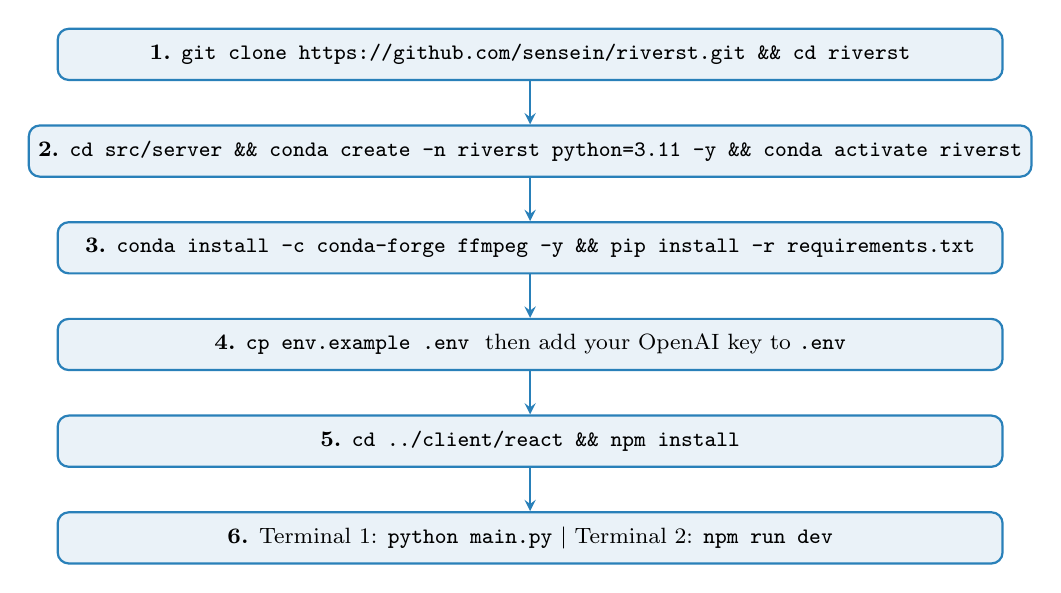
\begin{tikzpicture}[
    node distance=0.55cm,
    sbox/.style={rectangle, rounded corners, draw=kivablue, fill=kivablue!10, thick, minimum width=12cm, minimum height=0.65cm, align=left, font=\footnotesize},
    arr/.style={->, >=stealth, thick, color=kivablue}
]

\node[sbox] (s1) {\textbf{1.} \texttt{git clone https://github.com/sensein/riverst.git \&\& cd riverst}};
\node[sbox, below=of s1] (s2) {\textbf{2.} \texttt{cd src/server \&\& conda create -n riverst python=3.11 -y \&\& conda activate riverst}};
\node[sbox, below=of s2] (s3) {\textbf{3.} \texttt{conda install -c conda-forge ffmpeg -y \&\& pip install -r requirements.txt}};
\node[sbox, below=of s3] (s4) {\textbf{4.} \texttt{cp env.example .env} \ then add your OpenAI key to \texttt{.env}};
\node[sbox, below=of s4] (s5) {\textbf{5.} \texttt{cd ../client/react \&\& npm install}};
\node[sbox, below=of s5] (s6) {\textbf{6.} Terminal 1: \texttt{python main.py} \textbar\ Terminal 2: \texttt{npm run dev}};

\draw[arr] (s1) -- (s2);
\draw[arr] (s2) -- (s3);
\draw[arr] (s3) -- (s4);
\draw[arr] (s4) -- (s5);
\draw[arr] (s5) -- (s6);

\end{tikzpicture}
\end{frame}

\begin{frame}
\begin{center}
\vspace{0.5cm}
\Huge You're ready!

\vspace{0.8cm}

\Large Install $\rightarrow$ Pick avatar $\rightarrow$ Customize $\rightarrow$ Talk

\vspace{0.8cm}

\normalsize
\faGithub\ \url{https://github.com/sensein/riverst}

\vspace{0.3cm}

\faEnvelope\ Ask for help on Slack anytime
\end{center}
\end{frame}

\end{document}
